% Created 2018-06-25 Mo 13:07
% Intended LaTeX compiler: pdflatex
\documentclass[11pt]{scrartcl}
\usepackage[utf8]{inputenc}
\usepackage[T1]{fontenc}
\usepackage{graphicx}
\usepackage{grffile}
\usepackage{longtable}
\usepackage{wrapfig}
\usepackage{rotating}
\usepackage[normalem]{ulem}
\usepackage{amsmath}
\usepackage{textcomp}
\usepackage{amssymb}
\usepackage{capt-of}
\usepackage{hyperref}
\author{simon}
\date{\today}
\title{}
\hypersetup{
 pdfauthor={Simon Pfreundschuh},
 pdftitle={},
 pdfkeywords={},
 pdfsubject={},
 pdfcreator={Emacs 24.5.1}, 
 pdflang={English}}
\begin{document}

\setlength{\parindent}{0cm}

\section{Major points}

\subsection*{Review comment 1}

A major aspect of the study concerns the representation of the particle size
distribution which is retrieved by two free parameters (different from the 2
moments of the atmospheric model GEM used to provide the test scenes) and the
assumptions of the particle type. The difficulty of connecting atmospheric model
output to single scattering properties (which is one of the fundamental
assumptions) could be better explained. The motivation why the authors choose
their approach and why they test certain settings need to be discussed in the
beginning. Couldn’t Tab. 1 and 4 be combined and better explained which is used
for which purpose? Why is cloud ice the same and GEMsnow and GEMGraupel different
in both?

\subsubsection*{Author response:}

The authors agree with the reviewer that the rather arbitrary choice of
tested particles has been a weak spot of the study. To improve this,
the authors tried to come up with a more principled selection of particles
to test. The new selection is based on the particle properties described
in \citet{ekelund19} and covers a broader range of mass-size relationships
and scattering parameters. In particular, the GemSnow model has been removed
from the selection of test particles, because it does not cover small
ice particle sizes. The following paragraph has been added in Sect.~2.3 which discusses
the choice of the particle model and the difficulty connecting model output
with single scattering properties.
\vspace{1em}

\textit{The standard deviations in the covariance matrix have been deliberately
  chosen to be very loose in order avoid the introduction of constraining
  information that may be provided by the radiometer observations.}

\subsection*{Reviewer comment 2}

Although different parameterizations of the hydrometeor types are used to
study their effects, vertical changes (development of sedimenting particles)
are not considered. Similar polarization effects are not mentioned in the
discussion on particleshape. Otherwise the paper nicely discusses the different
aspects but in the end I ammissing a clear message on the outcome of the test
(choice of particle types). What isrecommended for the future?

\subsubsection*{Author response}

It is true that vertical changes in the particle shape are not considered in the
retrieval forward model. However, the retrieval forward model can adjust two
degrees of freedom of the PSD. This should allow represent sedimentation of particles,
which would lead to a decrease of the number density and an increase of the particle
size towards the base of the cloud.

Polarization effects are neglected in this study for several reasons. Firstly,
oriented scattering data has only recently become available. Secondly, the GEM
model does not provide any information on oriented particles.

To address the point of a missing recommendation on the best particle model, the
following recommendation based on the results obtained with the new selection of
particle shapes has been added to the manuscript.

\subsection*{Reviewer comment 3}

Not only the two moments of the ice PSD but further variables are retrieved and
their information content is nicely shown in Fig. 14. I am surprised that the
information on moisture is so low although information along three water vapor
lines is provided? This should at least in the upper atmosphere provide
information? Is it due to the choice of relative humidity which mainly depends
on temperature? I am also skeptical about the results of Fig. 16. Basically,
there should be no liquid for temperatures colder than 40 deg C (freezing) but
it even reference LWC goes up to 13 km? I would not support the statement on
L568 – where is the evidence? Similar L527 – Liquid water estimation within
mixed phase clouds is extremely difficult and if ICI and radar could really do
that together this would be worth a separate paper. To better understand the
information content, I suggest to plot the profiles of cumulative degrees of
freedom for the different retrievals as this could help interprete where and how
the synergy works.

\subsubsection*{Author response}

Regarding the information content on water vapor, a possible explanation is the
way relative humidity was calculated within ARTS. ARTS follows the method
proposed by \citet{}, which effectively interpolates between the relative
humidities w.r.t. water and ice. Since relative humidity was arctan-transformed
with a threshold value of 1.2, high relative humidities at low temperatures may
have lead to a vanishing of gradients and therefore a miscalculation of the
information content with respect to water vapor. This will of course be corrected
in the updated version of the manuscript. We have also produced the desired plot
of the cumulative degrees of freedom for both test scenes and display it here.
Since the cause for the low reported information content on water vapor has been
detected and corrected, the authors decided not include the figure in the manuscript
so as to not lengthen it further.

Regarding the retrieval of cloud liquid water (CLWC), it seems that the
ambiguous description of the figure has caused a misinterpretation of the
presented results. The field shown in the background is not the retrieved (CLCW)
but the retrieved density of ice and rain hydrometeors. The retrieved CLWC is
shown by the colored contours, so there is indeed a fairly good agreement
between the retrieved and the reference CLWC. To avoid this kind of confusion,
colorbars have been added to the figure and the caption clarified.

\subsection*{Reviewer comment 4}

4) The manuscript is rather lengthy making it difficult for the reader to
extract the majorpoints. I strongly suggest a) to move part of the analysis into
an appendix (, b) remove double statement (see minor comments, also the LWC plot)
and c) to remove figurecaption like information (for example L92 or “filled
contours”) from the text. The textmust make sense without looking at the figure.
Figure only support the statementsmade in the text. Lengthy descriptions such as
“The plot shows..” need to be avoided.

\subsubsection*{Author response}

The suggestions made by the reviewer will be followed by moving the analysis of
the second test scene to the appendix as well as following the other recommendations
made in the comment.

\section{Specific comments}
\subsection*{Reviewer comment 1}
L39:  Is sensitivity really the right word?   Range resolution is the main advantage –signal-to noise range depends on distance and hydrometeor distribution,

\subsubsection*{Author response}

We would like to argue that this is indeed the right word. As can be seen for
example in Fig.~4 in the manuscript, the 94-GHz cloud radar provides a
measurable cloud signal at $D_m$ and IWC values that are significantly lower
than those at which a signal can be observed in the passive observations.

\subsection*{Reviewer comment 2}

L48: MWI will also cover new spectral channels, e.g. 118 GHz

\subsubsection*{Author response}

To incorporate this information the corresponding sentence will be changed to:

\textit{MWI will complement ICI's observations with measurements at traditional
  millimeter wavelengths as well as a novel spectral band around the
  $118\ \unit{GHz}$ Oxygen line.}

\subsection*{Reviewer comment 2}

L62: “high-resolution” is always relative for a model. I would recommend avoiding this term and use Cloud resolving Model (CRM).

\subsubsection*{Author response}

The proposed improvement will be adopted in the revised version of the manuscript.
The sentence now reads:

\textit{The algorithm is applied to synthetic observations of cloud scenes from
  a cloud-resolving atmospheric model and used to further explore the synergies
  between the active and passive observations.}


\textit{}

\subsection*{Reviewer comment 3}

L68:  After you mention GPM (with scanning radar) it might be good to say that you are only looking at a nadir pointing radar (curtain).  The swath center came bit as a surprise.

\subsubsection*{Author response}

To incorporate the proposed improvement the corresponding sentence has been
modified as follows:

\textit{This work applies the concept of synergistic radar and sub-millimeter radiometer
retrievals to the upcoming ICI and MWI sensors by combining them with a
conceptual, nadir-pointing W-band cloud radar.}

\subsection*{Reviewer comment 4}

L70:  There has been quite some literature about combining active and passive MWusing a Bayesian framework which should be acknowledged, e.g. Grecu, M., & Olson,W. S. (2006), Johnson et al. (2012) , Munchak, S. J., & Kummerow

\subsubsection*{Author response}

Following the suggestion of the reviewer, the following paragraph will be added to the introduction:

\textit{
... has been
investigated \citep{evans05, jiang19}.

Combined retrievals using radar and passive radiometer observations, have also
been developed for the Tropical Rainfall Measuring Mission (TRMM,
\citet{kummerow98, grecu04}) and the Global Precipitation Measurement (GPM,
\cite{hou14, grecu16, munchak11}) mission. However, since the principal target
of these missions were liquid hydrometeors, they make use of sensors at
comparably low microwave frequencies, which provide only limited sensitivity to
frozen hydrometeors.

This work ...
}


\subsection*{Reviewer comment 5}

L84:  Test scenes have a grid resolution of 1 km horizontally.  As this is not the true model resolution I would have recommended to coarse sample the model data (maybe every 5th data point) and include more diverse profiles instead.  This might be especially interesting for the scatter plots.

\subsubsection*{Author response}

Not doing this.

The point raised by the reviewer is certainly correct. However, the decision to restrict simulations
to two test scenes was motivated by the computational costs of performing the retrievals. Furthermore,
the scatter plots in Fig.~10, that was unfortunately missing from the manuscript but is shown below,
shows that the scatter plots are similar for both test scenes. This certainly indicates that the
test scenes contain sufficient profile variability to be representative. 

\textit{}

\subsection*{Reviewer comment 6}

Motivation lacking:  “To perform RT simulations for each GEM profile the PSD needs to be diagnosed from the prognostic GEM variables, i.e. N and m..”

\subsubsection*{Author response}

To address another comment by another reviewer the paragraph containing the sentence
will be rewritten and the sentence removed.

\textit{ The prognostic parameters of the two-moment scheme are the slope and
  intercept parameters of the distribution, which are derived from the mixing
  ratios and number densities predicted by the GEM model. The third parameter of
  the PSD and the mass-size relationship of each hydrometeor class are set to
  fixed, class-specific values. The parameters of the mass-size relationships
  are given in Tab.~\ref{tab:species_parameters}. The masses of all ice
  particles in the model are assumed to scale with a power of three, which leads
  to high densities for large particles.}



\subsection*{Reviewer comment 7}

L92:“prognoses”   means   forward   in   time   -   you   mean   diagnosed,   calculated,determined..

\subsubsection*{Author response}

The  word will be replaced by derived in the updated version of the manuscript.

\textit{The four panels display the derived particle size distributions for the
  four frozen hydrometeor types together with renderings of the particle shapes
  used in the forward simulations.}


\subsection*{Reviewer comment 8}
L98: I find the term “horizontal and vertical scaling” strange – why not saying PSD shape is similar but scaling in respect to diameter and number density. At least definethe term clearly the first time that you use it or define a short for it.

\subsubsection*{Author response}
 
The proposed  change will be adopted in the updated version of the manuscript. The sentence has been changed
as follows:

\textit{
As these plots show, the
assumed particle size distributions across different ice species vary mostly in
their scaling with respect to size and concentration, whereas the function shape shows less
variability.}

In addition to this, also the following changes will be introduced in the manuscript in order
to make the wording consistent:


L. 176:

\textit{ The PSD of a hydrometeor species at a given height level is represented
  by two scaling parameters: The mass-weighted mean diameter $D_m$, which scales
  the size of the particles, and the normalized number density $N_0^*$, which
  scales the concentration of particles.}

L. 183:

\textit{ The retrieved scaling parameters of particle size and concentration,
  $D_m$ and $N_0^*$, are used as units for the axes of the plot so that the
  shape of the PSD becomes independent of the retrieved mass density and number
  concentration. }

L. 244:

\texit{The question that is addressed here is whether the combination of active
  and passive observations is able to constrain both the size and concentration
  of the ice particles in the cloud.}

L. 252:

\textit{ In the figure, the cloud signal is displayed in $D_m$-mass density
  space and thus shows how the measured passive cloud signal varies with size
  and concentration of particles in the cloud. }


L. 449:
\textit{The results show that the combined observations can simultaneously
  constrain the size and concentration of particles in the cloud.}


\subsection*{Reviewer comment 9}
L103: model test – be careful also at other instances that “model” can mean too manythings. Here I would say GEM test scenes.

\subsubsection*{Author response}

The proposed change will be adopted in the revised version of the manuscript by
changing the sentence as follows:

\textit{
The simulations apply the same microphysics scheme
as the GEM test scenes, which means that they use the same six hydrometeor classes
and PSD parametrizations.}


\subsection*{Reviewer comment 10}
L119: Need to clearly say that polarization effects are neglected though these can beseveral Kelvin, e.g.  Xie et al., 2015.  You ignore this effect but even consider noise reduction.

\subsubsection*{Author response}

In response to another reviewer's comment, we have decided to change the viewing
geometry assumed in the simulations to observations at nadir. Furthermore, the
second paragraph of Sect. 2.1.1 has been rewritten to clearly state the simplifying
assumptions made in the simulations. The paragraph now reads as follows:

\textit{In order to reduce the complexity of generating simulated observations, a number
of simplifications are applied to the viewing geometry and the radiative
transfer modeling. The beams of all three sensors are assumed to point at nadir
and to be perfectly coincident pencil beams. In this way, observations for the
GEM model scenes can be simulated by performing a single 1-dimensional radiative
transfer calculation for each profile. Moreover, multiple scattering effects in
the radar observations are neglected. The simulations therefore do not take into
account beam filling effects caused by atmospheric inhomogeneity across the
footprints of the different sensors. The incidence angles of the beams of ICI
and MWI will be around $53^\circ$ at the Earth's surface, so the simulations
performed here do not represent the viewing geometry of a space-borne
configuration involving ICI and MWI accurately. Realistic modeling of the
viewing geometry as well as multiple scattering effects in a variational
retrieval are currently not feasible at reasonable computational cost with the
tools used in this study. Assuming observations at nadir further allows neglecting
polarization effects, which can be several Kelvin at typical viewing geometries
of imager sensors \cite{xie15}. Since the focus of this study are the fundamental
synergies between the active and passive observations, this was deemed
sufficient for its scope. Moreover, these assumptions are justifiable for
air-borne observations, which adds practical relevance to the simulations.}



\subsection*{Reviewer comment 11}
L157-159: needs to be better motived, references?

\subsubsection*{Author response}

The $\chi^2$ value defined in the manuscript corresponds to the component of the OEM cost that
is related to the misfit in the observation vector. We use this value here as a heuristic
to asses the goodness of the retrieval fit. Since neither the a priori distribution nor the
observation error can be assumed to be Gaussian, applying a true $\Chi^2$-test is not really
meaningful. Similar applications can for example be found in \citet{duncan16}.

To state this more clearly in the manuscript, the following changes will be introduced:

\textit{The quantity $\chi^2_y$ corresponds to the squared error in the fitted
  observations weighted by the uncertainties in each channel. It should be noted
  that the quantity has no meaningful interpretation in terms of
  $\Chi^2$-statistic for the errors in the fitted observations since they will
  neither be independent (c.f. Chapter~12 in \cite{rodgers00}) nor Gaussian due
  to the presence of forward model error. The value is used here as a heuristic
  to quantify the goodness of the fit to the true observations.}


\subsection*{Reviewer comment 12}
L172: I doubt that the model has constant vertical resolution.  It will be better close to the surface and worse aloft. This should be mentioned than GEM is introduced.

\subsubsection*{Author response}

This is indeed the case. To make this clear to the reader the following sentence
is introduced in the paragraph describing the GEM model scenes:

\textit{The vertical resolution of the model scenes varies between 250
and $500\ \unit{m}$ below an altitude of $18\ \unit{km}$ and decreases
steadily above that.}

Furthermore, to address the Reviewer comment 13 a figure will be added to
the manuscript, which displays the model grid and the grids at which
the different retrieval quantities are retrieved.

\subsection*{Reviewer comment 13}

L 174: for all hydrometeor species of the model? It would be helpful to first
introduce all retrieval quantities – I was missing a motivation for the
paragraph around L195. How do you define the freezing layer (and later the
troposphere)? How do they vary in both test scenes? The model also likely has
supercooled liquid water above the freezing layer – how is this treated?

\subsubsection*{Author response}

In order to provide a better overview over the retrieval variables and
grid resolutions the following sketch of the different retrieval setups has
will be included in the revised version of the manuscript:

\begin{figure}
\centering
\includegraphics[width = 0.8\linewidth]{../plots/retrieval_sketch}
\caption{Illustration of the retrieval quantities and their respective retrieval
  grids. Grey, dashed lines show the resolution of the GEM model data while the
  filled circles represent the grid points of the different retrieval
  quantities. Panel (a) shows the configuration used in the radar-only and
  combined retrieval. Panel (b) shows the configuration used in the passive-only
  retrieval}
\label{fig:retrieval_sketch}
\end{figure}

The motivation for retrieving $N_0^*$ in log-space is that its a priori
distribution is more similar to a Log-normal rather than a Gaussian distribution
(see for example \textcite{delanoe15}). Since typical values for $D_m$ follow a
Gaussian distribution rather well these values are retrieved in linear space.

The handling of supercooled liquid in the GEM model scenes is similar to that
of all other hydrometeors and therefore not explicitly mentioned. In the retrieval,
liquid cloud is allowed to exist between the surface and the $240\ unit{K}$ isotherm
and thus also represents supercooled clouds.


\subsection*{Reviewer comment 13}

L 198:  Vertical resolution of retrieval grid:  Why 4 points?  The freezing layer must be very different for both cased. Maybe a sketch would be helpful as later on lines 230 thedifferent vertical resolutions for other variables is discussed?

\subsubsection*{Author response}

The choice of the number of grid points here was rather arbitrary but since it
was found to work acceptably well it was not investigated whether this is the
optimal choice.


\subsection{Reviewer comment}
L281: How do I know that Large Plate is the best performing model? Which parameter,plot, table does show that?

\subsubsection*{Author response}

This sentence is removed in the revised version of the manuscript.



\subsection*{Reviewer comment 14}
L283-L307: Can be shortened significantly

\subsubsection*{Author response}

Following the reviewers recommendations the section will be shortened and
now  reads as follows:

\textit{
Results of the retrieved water content for the first test scene are displayed in
Fig.~\ref{fig:results_a}. The corresponding results from the second test scene
are included in Appendix~\ref{app:results_b}. The reference water content is
defined here as the sum of the masses of the four frozen hydrometeor species in
the GEM model scenes.

The $\chi^2_y$ value of the different methods, displayed
in Panel (a), gives an indication of how well the retrievals were able to fit
the observations. For the radar-only retrieval, the values are far below 1
for most parts of the scene, while for the passive-only and combined retrieval
the around 1. This indicates that all methods fitted the observations well over
the whole scene except for the region around $3^\degree\ N$, where the cloud
is particularly thick.

In terms of IWP, all methods provide fairly good estimates of the reference IWP
with the combined retrieval consistently yielding the smallest deviations.
Larger differences between the methods are observed when comparing the retrieval
results in terms is IWC. While the vertical structure of the cloud is captured
only very roughly by the passive retrieval, it much better resolved by the
radar-only and the combined retrieval. On closer inspection, however, it becomes
evident that the radar-only retrieval deviates systematically from the reference
IWC in specific regions of the cloud, such as for example the upper part of the
cloud between $0^\circ N$ and $2^\circ N$. These deviations are corrected in
the results from the combined retrieval, although certain retrieval artifacts
are visible here.
}


\subsection*{Reviewer comment 15}
L332: There can I see that? Give figure?

\subsubsection*{Author response}

As part of the changes introduced to address the previous comment
this line will be removed from the manuscript.

\subsection*{Reviewer comment 16}
L325: The two paragraph here give similar information -> streamline

\subsubsection*{Author response}

To make the description of the results from the scatter plots more
concise the section will rewritten as follows:

\textit{
Not surprisingly, the results from the
passive-only retrieval exhibit the strongest deviations from the diagonal. Since
the passive channels alone contain only limited information on the vertical
distribution of ice in the atmosphere, the retrieval cannot be expected to yield
accurate results at the resolution considered here. Although rather weak, a
certain effect of the ice particle model on the retrieval results can be
observed. In particular, the GemCloudIce model leads to a systematic
underestimation of ice mass densities, which are less pronounced for the other
particle models.

In terms of overall accuracy, i.e. systematic deviations from the diagonal, no
clear differences between the three configurations are visible. The color-coding
reveals, however, that the radar-only retrieval is biased for specific
hydrometeor classes. This effect is less pronounced for the combined retrieval
and seem to be weaker also in the passive-only results. For Graupel, both the
radar-only and the combined retrieval perform badly but this due to the radar
signal saturating in the regions of the scene where Graupel is present (c.f.
Fig.~\ref{fig:overview} and Fig.~\ref{fig:observations_a}).

Results of all retrievals are affected by the choice of the ice particle model,
which can cause systematic deviations especially at high IWC values. For the
radar-only results these deviations are smallest for the LargeColumnAggregate,
whereas for the combined retrieval the LargePlateAggregate and 8-ColumnAggregate
yield the most accurate results.}


\subsection*{Reviewer comment 17}
L333-344: I would put this to the appendix

\subsubsection*{Author response}
We will follow the reviewers advice and put the analysis of the second test scene
into the appendix.

\subsection*{Reviewer comment 18}
L444: Here it needs to be made clearer how this goes beyond what GPM is doing.


\subsubsection*{Author response}

To clarify how our work goes beyond what GPM is doing the following paragraph
will be added to the manuscript:

\textit{The novelty of this work lies, for one part, in the application of ICI's
sub-millimeter channels, which sets it apart from the combined retrievals
developed for the TRMM and GPM missions. For the other part, it lies in the
development of a fully-consistent variational retrieval in which all retrieval
quantities are retrieved from the observations from all sensors simultaneously.
This allows comparing the retrieval to equivalent radar-only and passive-only
configurations and therefore a direct analysis of the synergies between the
active and passive observations.}

\subsection*{Reviewer comment 19}
L495:  “does not say much about the general validity of the assumption”.   Here you should dig in a bit more. What is the role of a priori and covariances?

\subsubsection*{Author response}

To extend the discussion of the role of the a priori assumptions in the retrieval
the corresponding paragraph will be modified as follows:

\textit{
  The a priori assumptions which were used in this study were similar but not
  identical to what is used in the DARDAR retrievals. Also here it should be
  noted, that the presented results should not be taken to be representative for
  the DARDAR product. Rather than this, the DARDAR a priori settings were chosen
  since they represent well established and validated assumptions for ice cloud
  retrievals and therefore should provide a reasonable starting point for the
  development of a combined cloud retrieval. Although the a priori assumptions
  work well for the first test scene they lead to systematic error in the second
  scene. The analysis in Fig.~\ref{fig:results_scatter} shows that the cause for
  this is the composition of the cloud. The a priori works well if the scene
  contains both snow and ice but causes systematic errors when this is not the
  case. The role of the a priori is to complement the observations with additional
  information in order to make the retrieval problem tractable. For the radar-only
  retrieval this means that the a priori determines how the information from a
  single range gate is distributed between the two degrees of freedom of the
  particle size distribution. Since the degrees of freedom vary more or less
  independently from each other, no a priori can fit for every possible cloud
  configuration.
}

\subsection*{Reviewer comment 20}
L560:  Rethink the bullet structure.  2.  Is not an independent result.  For each resultrefer to the part of the manuscript where you can clearly see that.  Especially result 3 should be detailed – how do ICI channel advance the currently available data?

\subsubsection*{Author response}

To improve the presentation of the conclusions, the bullet points will be removed
and the first paragraphs of the conclusions will be rewritten as follows:

\textit{The main conclusion from this work is that the combination of radar and
  sub-millimeter radiometer observations allows to constrain both the size
  as well as the concentration of frozen hydrometeors. The sensitivity of
  the combined observations to the microphysics of the cloud reduced the
  median bias in the retrieved IWC from more than $50\ \%$ in the radar-only
  to less than $10\ \%$ for suitable choices of the particle model (Fig.~\ref{fig:boxes}).

  Our results particularly highlight the importance of sub-millimeter observations
  for combined retrievals of frozen hydrometeors. While observations at currently
  available microwave frequencies provide only limited complementary information
  to the radar observations, it is mainly the frequencies above $200\ \unit{GHz}$
  that provide additional information on cloud microphysics (Fig.~\ref{contours})
  for

  Moreover it has been found that the combination of radar and passive microwave
  observations may help the retrieval of mixed-phase clouds. Since the role of
  these clouds in the climate of the arctic are an active topic of study, the use
  of combined sub-mm/radar observations should be further investigated.}


\subsection*{Reviewer comment 21}
Fig.  3: Is it really worth having the slightly different size distribution shapes for frozen and liquid? Isn’t there a stronger difference between different frozen hydrometeors

\subsubsection*{Author response}

We agree with the reviewer that the slightly different size distributions shapes likely do
not affect the retrieval significantly. The choice of the PSD parameters for liquid
hydrometeors was made rather arbitrarily, but since the retrieval was found to work
the effect of the PSD parameters has not been investigated further.

\subsection*{Reviewer comment 22}
Figures 7 and 8:  I’m not sure why these are separate figures – it seems like allpanels could fit on one page.

\subsubsection*{Author response}

Figures 7 and 8 will be combined into a single figure in the updated manuscript.

\subsection*{Reviewer comment 23}
Fig. 4 and also in text: “cloud signal” say that this is dTB.

\subsubsection*{Author response}

Following the reviewers recommendation, the passive cloud signal is now
referred to in the text as $\Delta T_B$ and the radar signal as
$\text{dBZ}_\text{max}$. The corresponding paragraph will also be changed
to make it more concise:

\textit{
The question that is addressed here is whether the combination of active and
passive observations is able to constrain both the size and concentration of the
ice particles in the cloud. To investigate this, the $N_0^*$ and $D_m$
parameters of the homogeneous cloud layer are varied and observations of the
cloud layer are simulated. The passive cloud signal ($\Delta T_B$) is the
difference between the cloudy- and clear-sky  brightness temperatures. The
signal in the active observations is here defined as the maximum in the measured
profile of radar reflectivity $\text{dBZ}_\text{max}$. Figure~\ref{fig:contoures}
displays the contours of $\Delta T_B$ and $\text{dBZ}_\text{max}$ with respect
to $D_m$ and the clouds IWC, which is proportional to $N_0^*$:
\begin{align}
m = \frac{\pi \rho}{4 ^ 4}N_0^* D_m^4,
\end{align}
where, $\rho$ is the density of ice.

  }


The proposed change will be adopted in the updated version of the manuscript.

\subsection*{Reviewer comment 24}
Fig. 5: Can you add freezing layer height?

\subsubsection*{Author response}
Freezing layer has been added to Fig.~5, which now looks as follows:

\begin{figure}
\centering
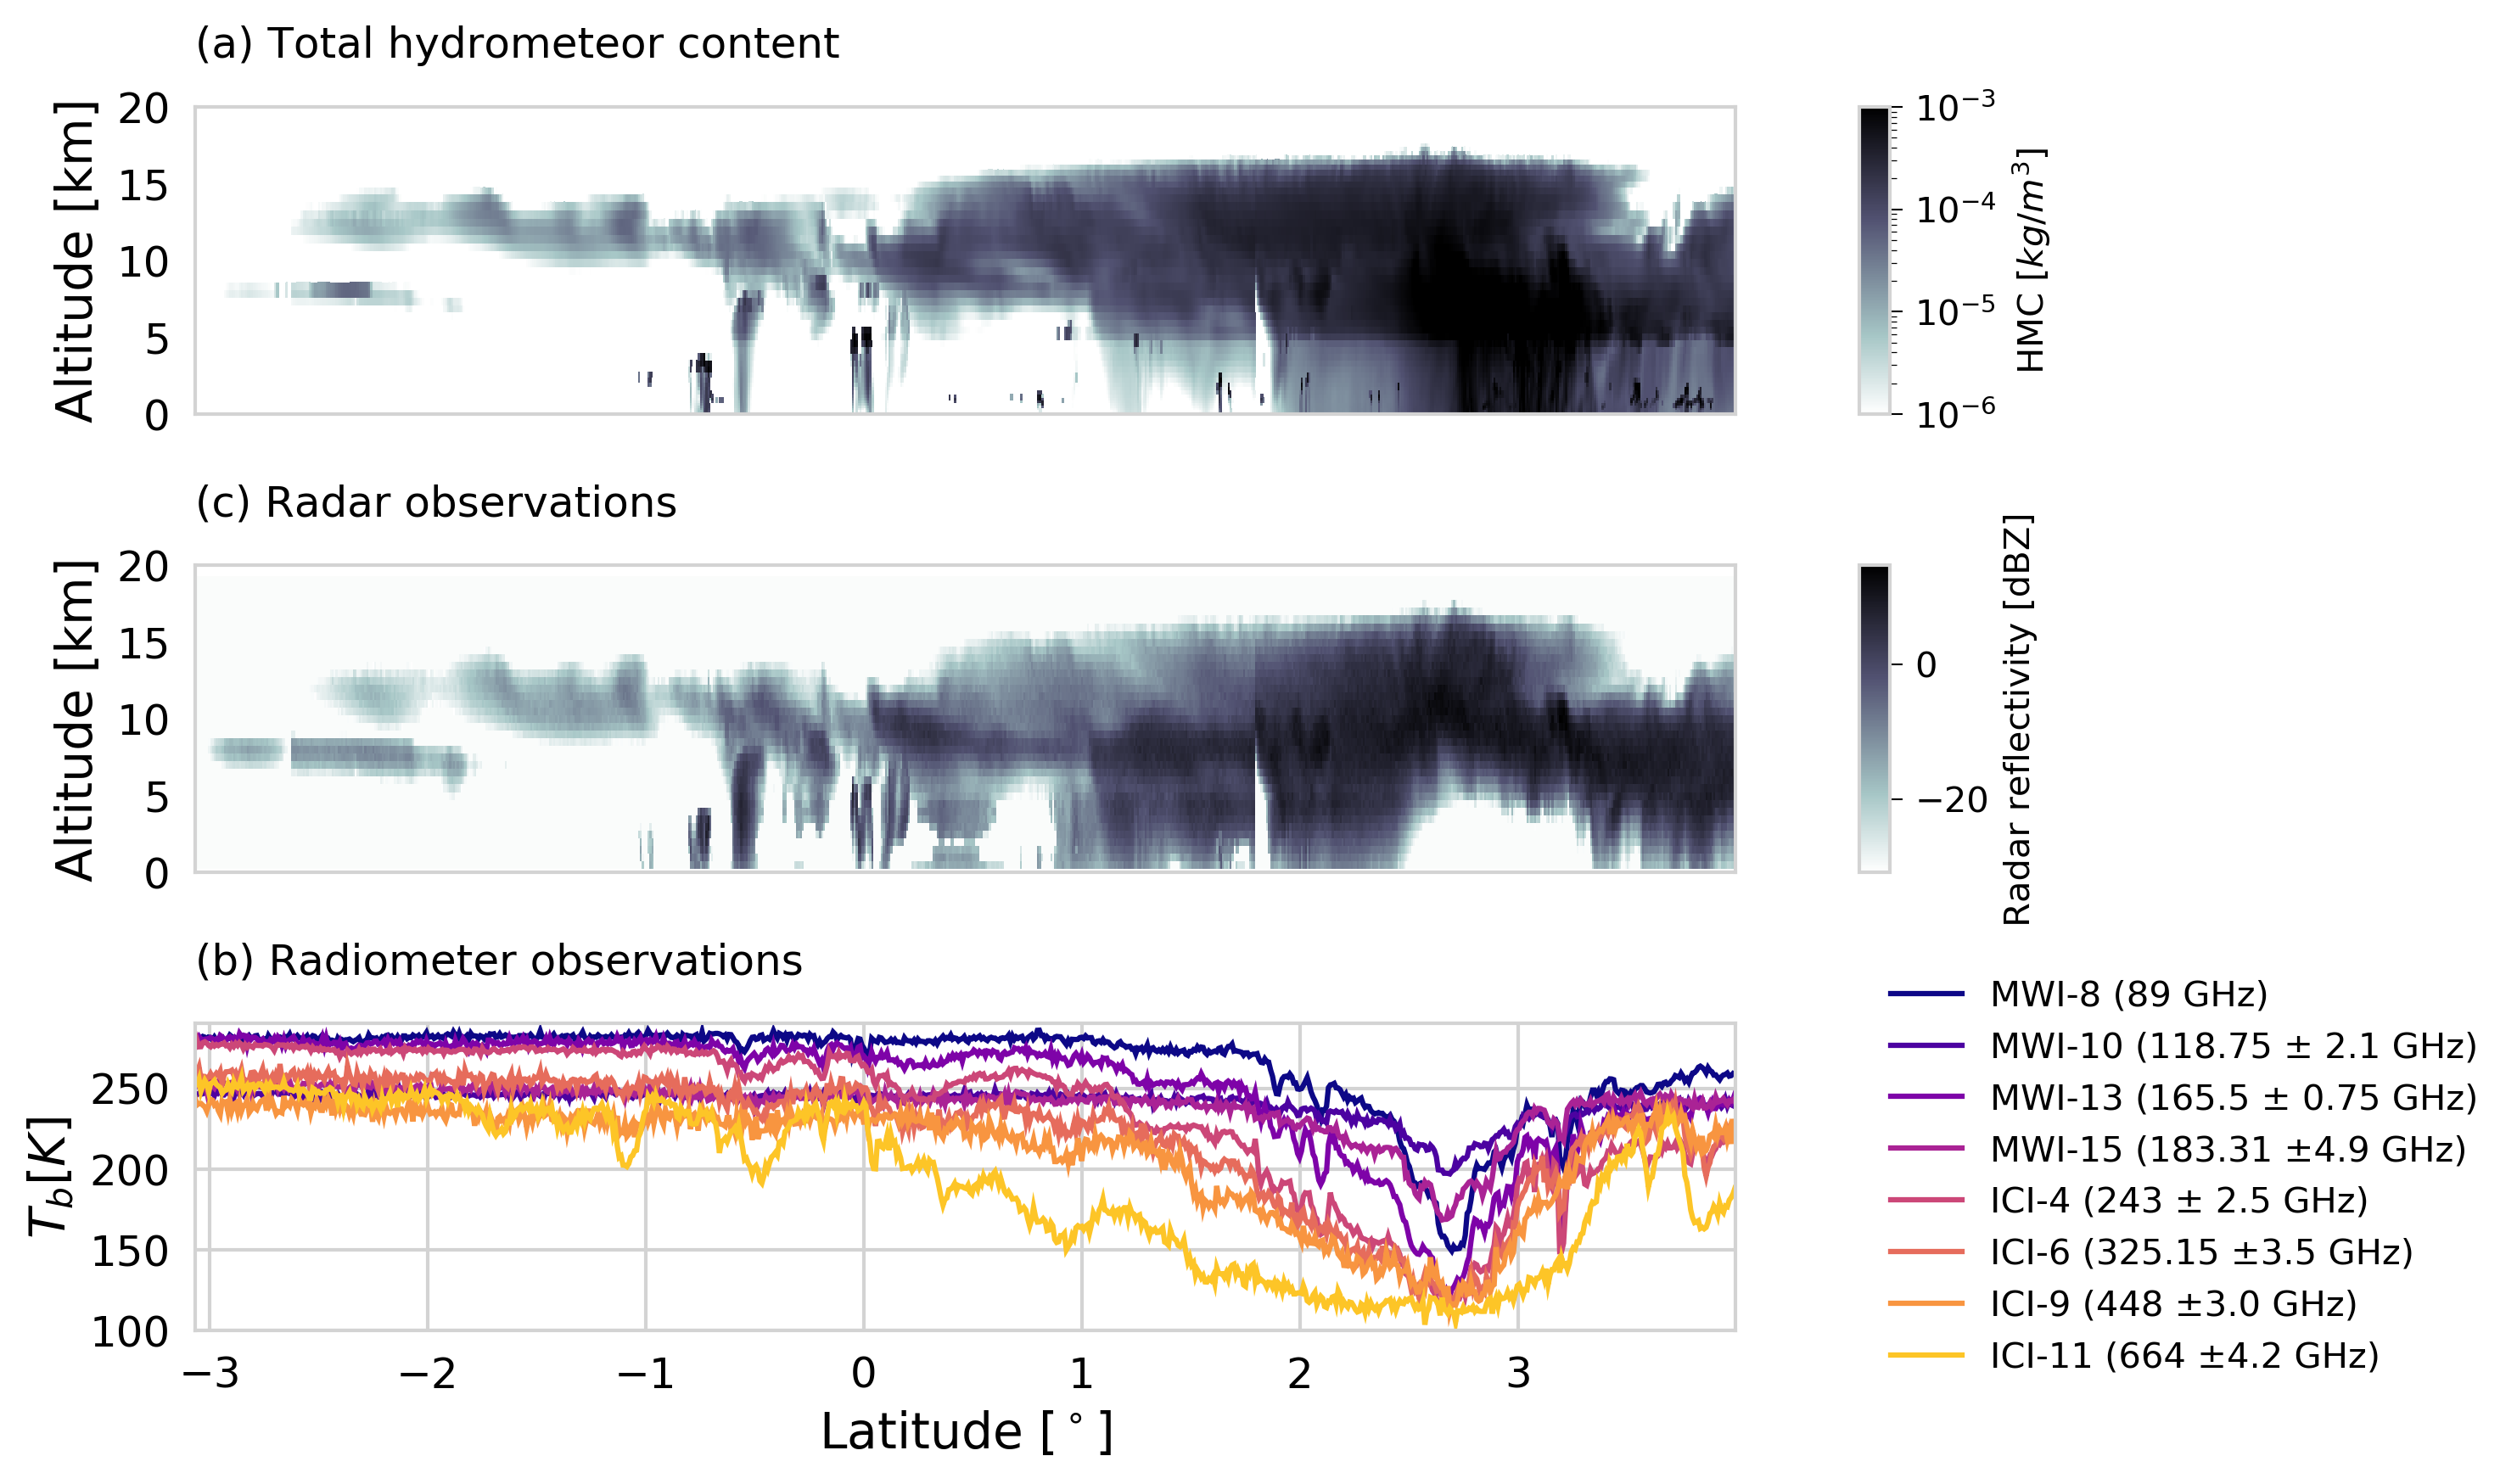
\includegraphics[width = 0.8\textwidth]{../plots/observations_a.png}
\caption{Total hydrometeor content (HMC) and simulated observations for the first test
  scene. Panel (a) displays the total hydrometeor content in the scene, i.e. the
  sum of the mass densities of all hydrometeor species of the GEM model. Panel
  (b) shows the simulated radar reflectivities. Panel (c) displays the simulated
  brightness temperatures for a selection of the channels of the MWI and ICI
  radiometers.}
\label{fig:observations_a}
\end{figure}


\subsection*{Reviewer comment 25}
Fig.  6:  It would be nice to see the absolute values of IWP somewhere.  Maybe youcould add another time series with IWP as the sum of the different components such that the reader can see where the different categories (cloud, graupel, snow and hail) contribute most?

\subsubsection*{Author response}

To address the reviewers request the figure will be modified as follows:

\begin{figure}
\centering
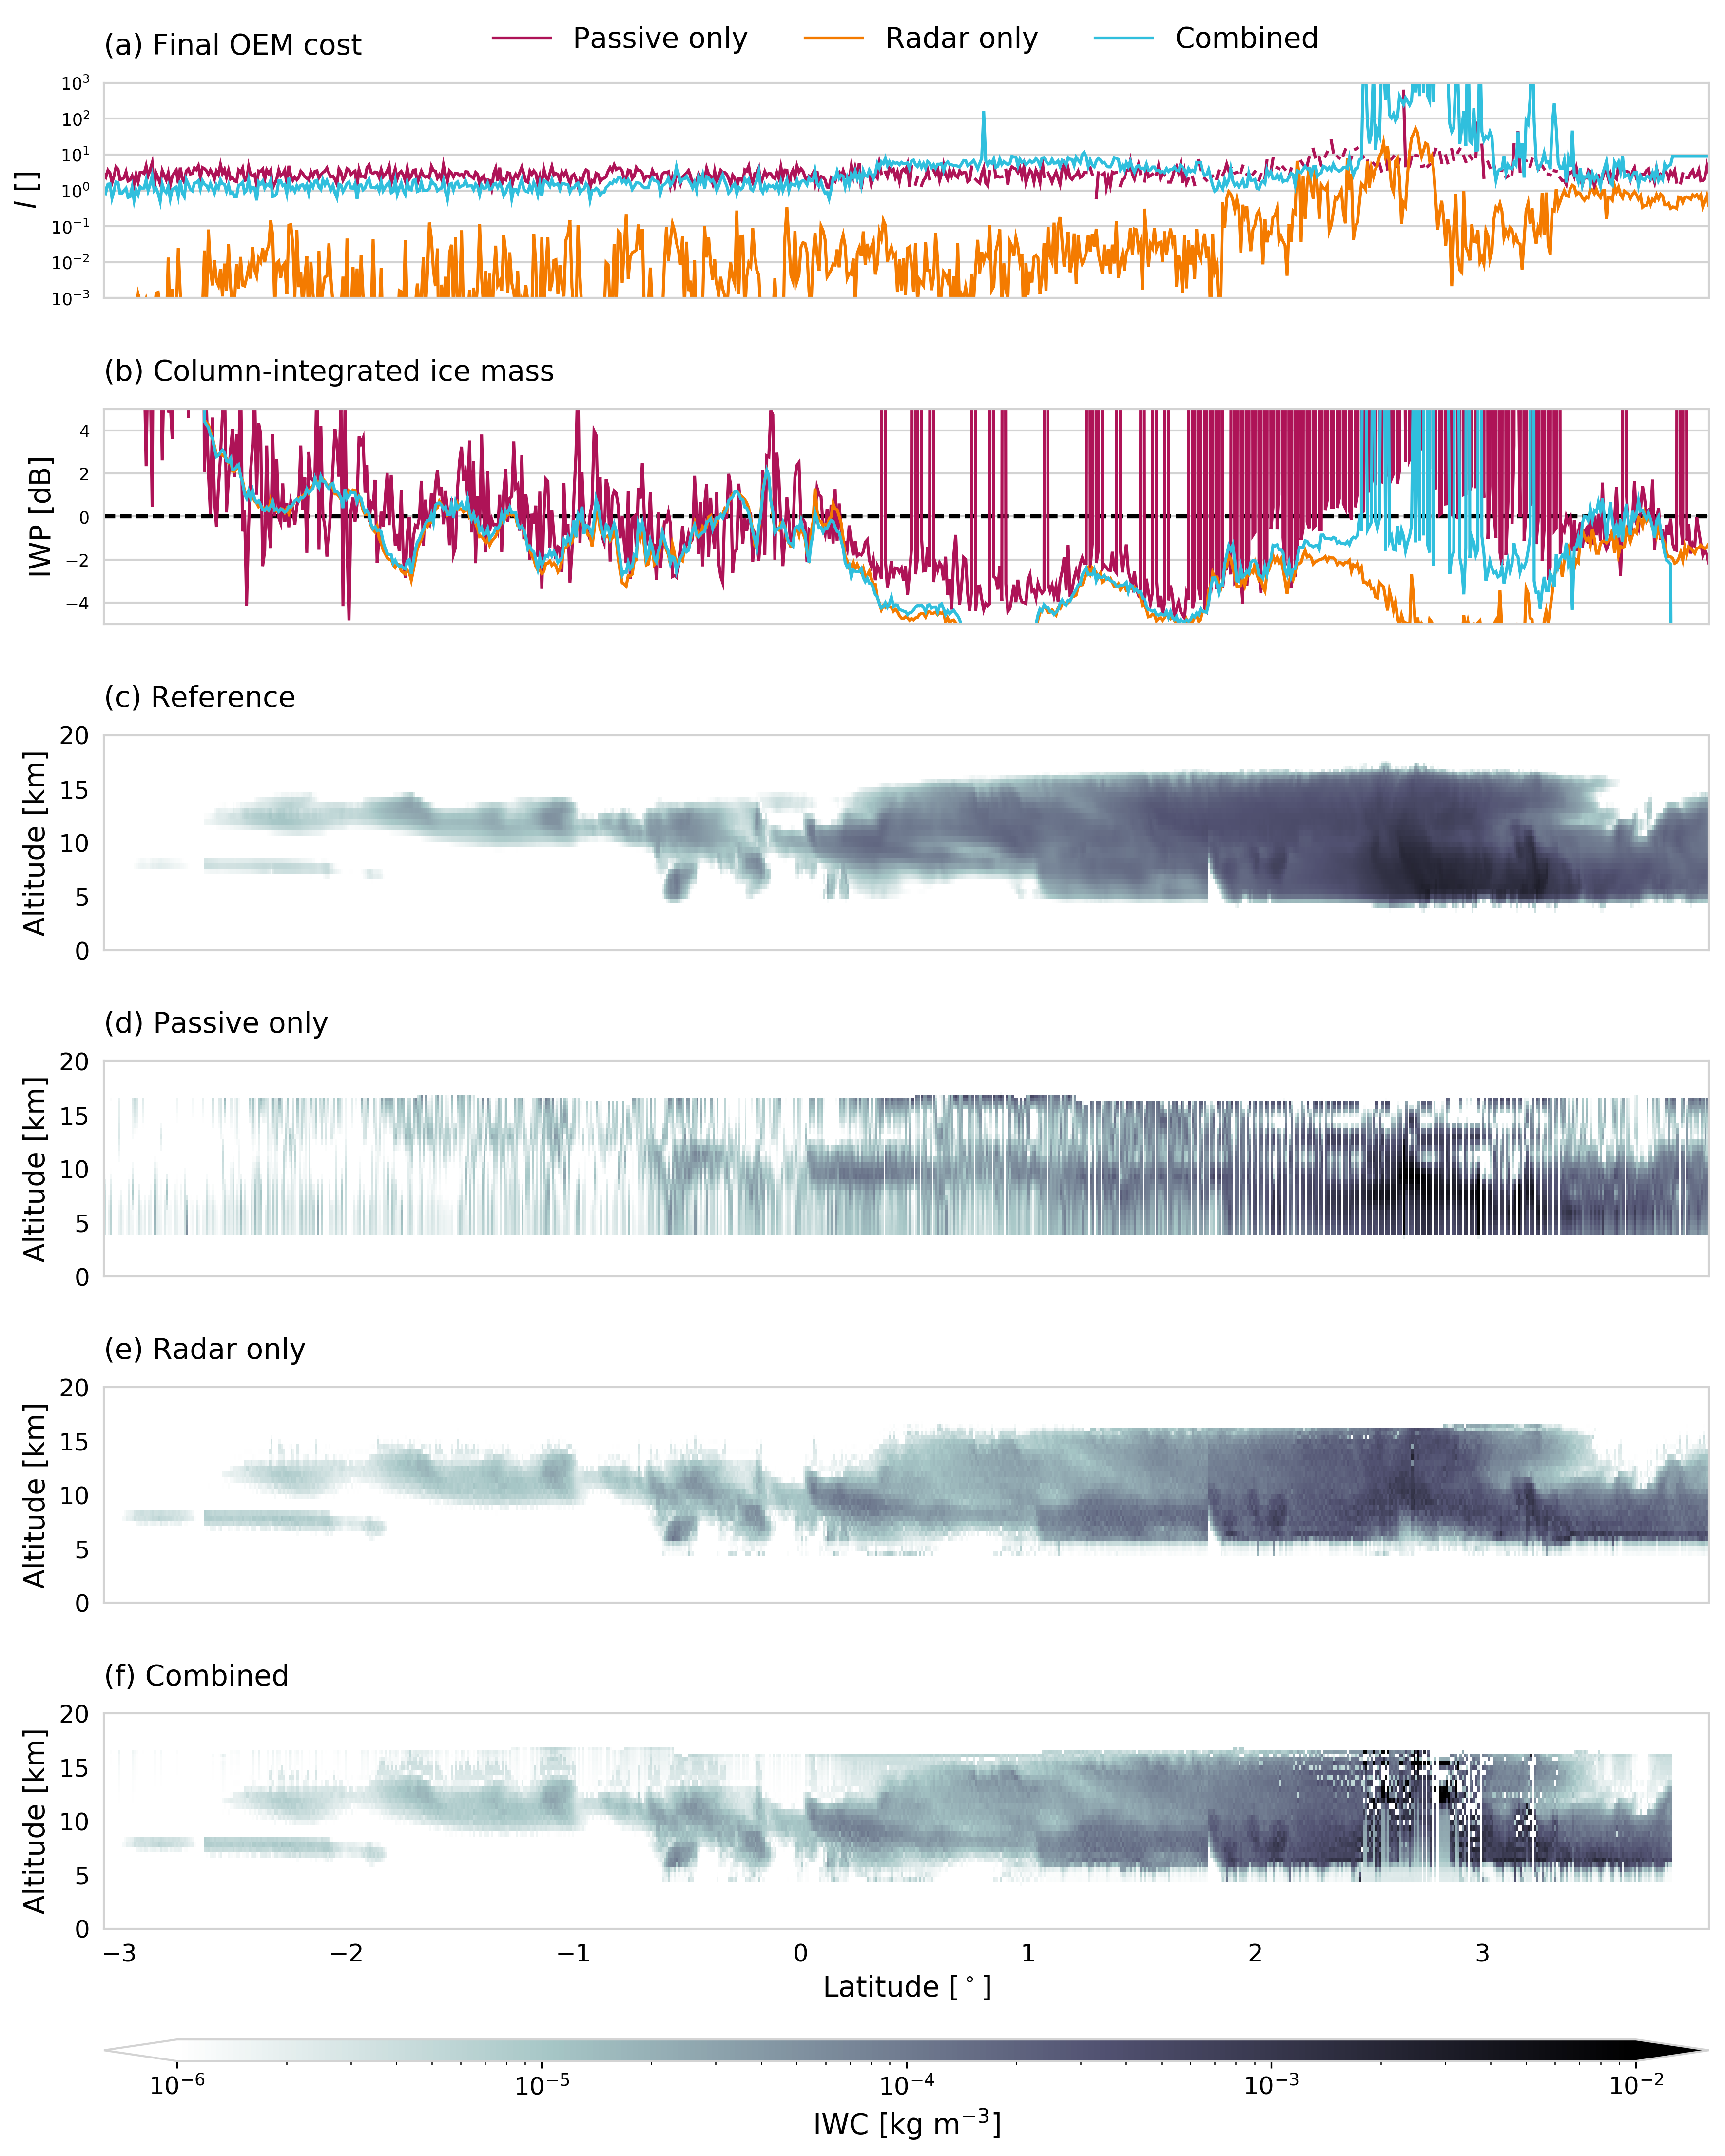
\includegraphics[width = 0.8\textwidth]{../plots/results_a_LargePlateAggregate.png}
\caption{Results of the ice hydrometeor retrieval for the first test scene.
  Panel (a) displays the value of the $\chi^2_y$ diagnostic normalized by the
  dimension of the measurement space of the corresponding retrieval. Panel (b)
  displays retrieved IWP in dB relative to the reference IWP. Panel (c) shows
  the reference IWC from the model scene. Panel (d), (e) and (f) display the
  retrieval results for the passive-only, radar-only and combined retrieval,
  respectively.}
\label{fig:results_a}
\end{figure}


\subsection*{Reviewer comment 26}
Fig.  7:  I think it is retrieved vs.  truth.  The word following is not really exact.  Why not put 7 and 8 together?

\subsubsection*{Author response}

The following will be corrected and Fig. 7 and 8 will be combined into 1 to look as follows:

\begin{figure}
\centering \includegraphics[width = 0.8\textwidth]{../plots/results_scatter.png}
\caption{Retrieved IWC plotted against reference IWC for the tested retrieval
  configurations. Each row shows the retrieval results for the particle shape
  shown in the first panel. The following panels show the retrieval results for
  the passive only (first column), the radar only (second column) and the
  combined retrieval (third column). Markers are colored according to the
  prevailing hydrometeor type at the corresponding grid point in the test
  scene. Due to their sparsity, markers corresponding to graupel are drawn at
  twice the size of the other markers.}
\label{fig:results_scatter_a_1}
\end{figure}

\subsection*{Reviewer comment 27}
Fig. 9: Could go to the appendix

\subsubsection*{Author response}
Fig.~9 will be moved to the appendix.

\subsection*{Reviewer comment 28}
Fig. 10 I only see the caption???

\subsubsection*{Author response}
Fig. 10 was unfortunately missing from the manuscript and as the responsible author I would like
to apologize for this mistake. The figure has been included in the appendix with the analysis
of the second test scene.

\subsection*{Reviewer comment 29}
Tab. 1. Assumed particle model information for each hydrometeor class given by GEMmodel. In fact it could be good to combine it

\subsubsection*{Author response}
Unfortunately we are not sure how to interpret this comment.

\section*{Grammar, typos and reformulations}

The authors would like to thank the reviewer for the additional comments which all
will be integrated into the updated manuscript.

\end{document}
